\documentclass[]{article}

\usepackage{mathtools,mathrsfs,url,fancyhdr, graphicx,amssymb,amsthm,tensor}
\usepackage[none]{hyphenat}
\renewcommand{\headrulewidth}{0pt}
\newcommand\numberthis{\addtocounter{equation}{1}\tag{\theequation}}
\fancyhead[L]{}
\fancyhead[C]{
	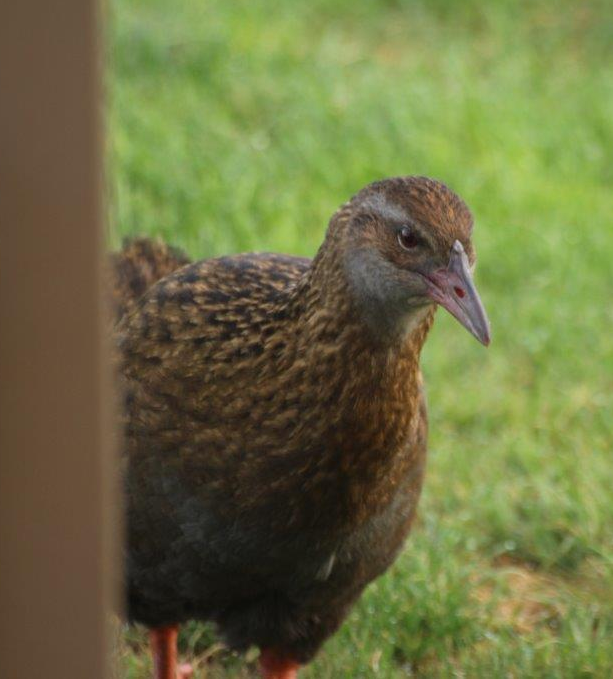
\includegraphics[width=2cm]{weka.png}
}


\graphicspath{ {images/} }
\newcommand{\Lagr}{\mathscr{L}}
\pagestyle{plain}

%opening
\title{Introduction into General Relativity\\Assignment 4\\Computing Christoffel Symbols}
\author{Simon Crase}

\newtheorem{theorem}{Lemma}

\begin{document}

\maketitle
\thispagestyle{fancy}
\raggedright
\begin{abstract}

Show that from the variational equation $0=\delta \int d \tau g_{\mu\nu}[z(\tau)] \dot{z^{\mu}} \dot{z^{\nu}} $ follows the relation $\ddot{z^{\mu}}+\Gamma\indices{^\mu_\nu_\alpha} \dot{z^{\nu}} \dot{z^{\alpha}}=0$.
 This observation frequently gives a practical way to calculate Christoffel symbols.
Using this method find Christoffel symbols for the metric
$ds^2 = e^{\nu(r,t)} dt^2 - e^{\lambda(r,t)} dr ^ 2 -r^2 d\Omega^2$
\end{abstract}

\section{Variational Equation}
\begin{theorem} [Geodesic]
	\label{lemma:geodesic}
	$0=\delta \int d \tau g_{\mu\nu}[z(\tau)] \dot{z^{\mu}} \dot{z^{\nu}} \implies \ddot{z^{\mu}} + \Gamma\indices{^\mu_\nu_\alpha} \dot{z^{\nu}} \dot{z^{\alpha}}=0$
\end{theorem}
\begin{proof}
	I shall assume that the integral is being computed over the interval $[-\infty,\infty]$. If not the proof is still valid \emph{mutatis mutandis}
	
	Consider changing the integral $\int_{-\infty}^{\infty} d \tau g_{\mu\nu}[z(\tau)] \dot{z^{\mu}} \dot{z^{\nu}}$ by replacing $z(\tau)$ by $z(\tau)+\eta(\tau)$, where $\eta(\pm\infty)=0$ and  $\eta$ is small. Then the integral becomes
	\begin{align*}
	&\int_{-\infty}^{\infty} d \tau  g_{\mu\nu}[z(\tau)+\eta(\tau)] ( \dot{z^{\mu}}+ \dot{\eta^{\mu}}) ( \dot{z^{\nu}}+ \dot{\eta^{\nu}})\\
	=&\int_{-\infty}^{\infty} d \tau g_{\mu\nu}[z(\tau)] \dot{z^{\mu}} \dot{z^{\nu}} + \int_{-\infty}^{\infty} d \tau \frac{\partial g_{\mu\nu}[z(\tau)]}{\partial z^{\alpha}} \dot{z^{\mu}} \dot{z^{\nu}} \eta^{\alpha}\\
	+&\underbrace{2\int_{-\infty}^{\infty} d \tau   g_{\mu\nu}[z(\tau)] \dot{\eta^{\mu}} \dot{z^{\nu}}}_\text{Since $g_{\mu\nu}=g_{\nu\mu}$}  + O(\eta^2) \numberthis \label{eq:var}
	\end{align*}
	We introduce a new symbol, $\Delta_{\eta}$, for the change in the integral caused be $\eta$. From (\ref{eq:var}).
	\begin{align*}
	\Delta_{\eta} \int_{-\infty}^{\infty} d \tau g_{\mu\nu}[z(\tau)] \dot{z^{\mu}} \dot{z^{\nu}} \triangleq& \int_{-\infty}^{\infty} d \tau  g_{\mu\nu}[z(\tau)+\eta(\tau)] ( \dot{z^{\mu}}+ \dot{\eta^{\mu}}) ( \dot{z^{\nu}}+ \dot{\eta^{\nu}}) -\int_{-\infty}^{\infty} d \tau g_{\mu\nu}[z(\tau)] \dot{z^{\mu}} \dot{z^{\nu}}\\
	=&\int_{-\infty}^{\infty} d \tau \frac{\partial g_{\mu\nu}[z(\tau)]}{\partial z^{\alpha}} \dot{z^{\mu}} \dot{z^{\nu}} \eta^{\alpha}+2\underbrace{\int_{-\infty}^{\infty} d \tau   g_{\mu\nu}[z(\tau)] \dot{\eta^{\mu}} \dot{z^{\nu}}}_\text{Integrate this term by parts} + O(\eta^2) \\
	=&\int_{-\infty}^{\infty} d \tau \frac{\partial g_{\mu\nu}[z(\tau)]}{\partial z^{\alpha}} \dot{z^{\mu}} \dot{z^{\nu}} \eta^{\alpha}-2\underbrace{\int_{-\infty}^{\infty} d \tau  \eta^{\mu} \frac{ \partial (g_{\mu\nu}[z(\tau)] \dot{z^{\nu}})}{\partial \tau}}_\text{Using $\eta(\pm\infty)=0$} + O(\eta^2)\\
	=&\int_{-\infty}^{\infty} d \tau \big[\frac{\partial g_{\mu\nu}[z(\tau)]}{\partial z^{\alpha}} \dot{z^{\mu}} \dot{z^{\nu}}-2\frac{ \partial (g_{\alpha\nu}[z(\tau)] \dot{z^{\nu}})}{\partial \tau} \big]\eta^{\alpha} \\
	+& O(\eta^2) \numberthis \label{eq:delta}
	\end{align*}
	Combining with the hypothesis, $0=\delta \int_{-\infty}^{\infty} d \tau g_{\mu\nu}[z(\tau)] \dot{z^{\mu}} \dot{z^{\nu}}$, we see that $\Delta_{\eta} \int_{-\infty}^{\infty} d \tau g_{\mu\nu}[z(\tau)] \dot{z^{\mu}} \dot{z^{\nu}}=0 \text{ }\forall \text{ (suitable) } \eta$, which is true \emph{if and only if the integrand is itself zero.}
	\begin{align*}
	0=&\frac{\partial g_{\mu\nu}[z(\tau)]}{\partial z^{\alpha}} \dot{z^{\mu}} \dot{z^{\nu}}-2\frac{ \partial (g_{\alpha\nu}[z(\tau)] \dot{z^{\nu}})}{\partial \tau}\\
	=&\frac{\partial g_{\mu\nu}[z(\tau)]}{\partial z^{\alpha}} \dot{z^{\mu}} \dot{z^{\nu}}-2\frac{ \partial g_{\alpha\nu}[z(\tau)] }{\partial \tau}\dot{z^{\nu}}-2g_{\alpha\nu}[z(\tau)] \ddot{z^{\nu}}\\
	=&\frac{\partial g_{\mu\nu}[z(\tau)]}{\partial z^{\alpha}} \dot{z^{\mu}} \dot{z^{\nu}}-2\frac{ \partial g_{\alpha\nu}[z(\tau)] }{\partial z^{\mu}}\dot{z^{\mu}}\dot{z^{\nu}}-2g_{\alpha\nu}[z(\tau)] \ddot{z^{\nu}} \numberthis \label{eq:ode1}
	\end{align*}
	Raising the index $alpha$ in (\ref{eq:ode1})
	\begin{align*}
	0=& g^{\beta\alpha} g_{\alpha\nu}\ddot{z^{\nu}} + g^{\beta\alpha} \frac{\partial g_{\alpha\nu}}{\partial z^{\mu}} \dot{z^\nu} \dot{z^\mu} - g^{\beta\alpha} \frac{1}{2} \frac{\partial g_{\mu\nu}}{\partial z^{\alpha}} \dot{z^{\mu}} \dot{z^{\nu}}\\
	=& \ddot{z^{\beta}} + g^{\beta\alpha} \frac{\partial g_{\alpha\nu}}{\partial z^{\mu}} \dot{z^\mu} \dot{z^\nu} - g^{\beta\alpha} \frac{1}{2} \frac{\partial g_{\mu\nu}}{\partial z^{\alpha}} \dot{z^{\mu}} \dot{z^{\nu}}\\
	=& \ddot{z^{\beta}} + g^{\beta\alpha} \bigg[\frac{\partial g_{\alpha\nu}}{\partial z^{\mu}}-\frac{1}{2} \frac{\partial g_{\mu\nu}}{\partial z^{\alpha}} \bigg]   \dot{z^\mu} \dot{z^\nu} \\
	=& \ddot{z^{\beta}} + \frac{1}{2} g^{\beta\alpha} \bigg[\frac{\partial g_{\alpha\nu}}{\partial z^{\mu}} + \frac{\partial g_{\alpha\mu}}{\partial z^{\nu}} -\frac{\partial g_{\mu\nu}}{\partial z^{\alpha}} \bigg]   \dot{z^\mu} \dot{z^\nu} \numberthis \label{eq:ode2}	
	\end{align*}
	Equation (\ref{eq:ode2}) follows by interchanging $\mu$ and $\nu$ in the 2nd term and in $\dot{z^\mu} \dot{z^\nu}$. From \cite{akhmedev2016}
    \begin{align*}
    \Gamma\indices{^\mu_\nu_\alpha} \triangleq \frac{1}{2}g^{\mu\beta} \bigg(\partial_{\nu}g_{\alpha\beta} +\partial_{\alpha}g_{\beta\nu} - \partial_{\beta}g_{\nu\alpha}\bigg)
    \end{align*}
    We permute the indices $\begin{pmatrix}
    \beta & \alpha & \nu & \mu \\
    \alpha & \nu & \mu & \beta
    \end{pmatrix}$ to obtain:
    \begin{align*}
     \Gamma\indices{^\beta_\mu_\nu} = \frac{1}{2}g^{\beta\alpha} \bigg(\partial_{\mu}g_{\nu\alpha} +\partial_{\nu}g_{\alpha\mu} - \partial_{\alpha}g_{\mu\nu}\bigg)
    \end{align*}
    Substituting in (\ref{eq:ode2}) gives (\ref{eq:ode3}), which is the desired result, up to a relabelling.
    \begin{align*}
    \ddot{z^{\beta}} + \Gamma\indices{^\beta_\mu_\nu}   \dot{z^\mu} \dot{z^\nu} =0 \numberthis \label{eq:ode3}
    \end{align*}
\end{proof}
\section{Calculating the Christoffel Symbols}
Substituting for $d\Omega^2$ as in \cite{akhmedev2016}.
\begin{align*}
ds^2 =& e^{\nu(r,t)} dt^2 - e^{\lambda(r,t)} dr ^ 2 -r^2 d\Omega^2\\
=& e^{\nu(r,t)} dt^2 - e^{\lambda(r,t)} dr ^ 2 -r^2 d\theta^2 - r^2 sin^{2}\theta d\phi^2 \\
=& e^{\nu(z^0,z^1)} (dz^0)^2 - e^{\lambda(z^0,z^1)} (dz^1) ^ 2 -(z^1)^2 (dz^2)^2 - (z^1 sin(z^2))^2  (dz^3)^2 \numberthis \label{eq:metric}
\end{align*}
Where we have renamed the variables: $t\rightarrow z^0; r\rightarrow z^1; \theta\rightarrow z^2; \phi \rightarrow z^3,$ and also reordered the variables in functions $\lambda$ and $\nu$. We write $\nu_0$ for $\partial_0\nu=\frac{\partial\nu}{\partial t},$ etc.  To minimize the risk of confusing superscripts, I shall use brackets when an expression is squared, e.g. $(\dot z^3)^2$ denotes the square of $\dot z^3$ or of $\dot \phi$.

Lemma \ref{lemma:geodesic} gives an expression for the Geodesic arising from the metric (\ref{eq:metric}), and Lagrange's equation gives another. We intend to calculate the Christoffel symbols by comparing the two expressions. That is, we will look for a curve $z(\tau)$ satisfying.
\begin{align*}
\delta \int d\tau \underbrace{\big[e^{\nu(z^0,z^1)} (\dot z^0)^2 - e^{\lambda(z^0,z^1)} (\dot z^1) ^ 2 -(z^1)^2 (\dot z^2)^2 - (z^1 sin(z^2))^2  (\dot z^3)^2\big]}_{=L\text{, say}}=0 \numberthis \label{eq:L}
\end{align*}
The curve can be found by solving the well-known Euler-Lagrange equations, \cite{wiki_lagrange}
\begin{align*}
\frac{d}{d\tau}\big(\frac{\partial L}{\partial \dot z^\mu}\big)-\frac{\partial L}{\partial z^\mu}=0 \numberthis \label{eq:EL}
\end{align*}
Substituting L from (\ref{eq:L}) in (\ref{eq:EL}) for $z^0$
\begin{align*}
0=&\frac{d}{d\tau}\big(\frac{\partial L}{\partial \dot z^0}\big)-\frac{\partial L}{\partial z^0}\\
= & \frac{d}{d\tau}\big(2 e^{\nu(z^0,z^1)}\dot z^0\big) - \frac{\partial L}{\partial z^0}\\
=& 2 e^\nu \big[\nu_0 (\dot z^0)^2 + \nu_1 \dot z^0 \dot z^1 +\ddot z^0\big]- e^{\nu}\nu_{0} (\dot z^0)^2 + e^{\lambda} \lambda_0 (\dot z^1)^2\\
=& e^\nu \big[2\ddot z^0+ \nu_0 (\dot z^0)^2 + 2\nu_1 \dot z^0 \dot z^1 + e^{\lambda-\nu} \lambda_0 (\dot z^1)^2\big]
\end{align*}
\begin{align*}
\ddot z^0+ \frac{1}{2}\nu_0 (\dot z^0)^2 + \frac{1}{2} \nu_1 \dot z^0 \dot z^1 + \frac{1}{2} \nu_1 \dot z^1 \dot z^0+ \frac{1}{2} e^{\lambda-\nu} \lambda_0 (\dot z^1)^2=0
\end{align*}
Comparing with (\ref{eq:ode3}) we see.
\begin{align*}
\Gamma\indices{^0_0_0} =& \frac{1}{2}\nu_0\\
=& \frac{1}{2}\partial_t \nu \numberthis \label{eq:C000}\\
\Gamma\indices{^0_1_0} =\Gamma\indices{^0_0_1} =& \frac{1}{2}\nu_1\\
=& \frac{1}{2} \partial_r \nu \numberthis \label{eq:C010}\\
\Gamma\indices{^0_1_1} =& \frac{1}{2}e^{\lambda-\nu}\nu_0\\
=& \frac{1}{2}e^{\lambda-\nu}\partial_t \numberthis \label{eq:C011} \nu
\end{align*}

Similarly for $z^1$
\begin{align*}
0=&\frac{d}{d\tau}\big(\frac{\partial L}{\partial \dot z^1}\big)-\frac{\partial L}{\partial z^1}\\
=&\frac{d}{d\tau}\big(-2e^{\lambda}\dot z^1\big)-\frac{\partial L}{\partial z^1}\\
=&-2e^\lambda \big[\ddot z^1 + \lambda_0\dot z^0\dot z^1 + \lambda_1 (\dot z^1)^2\big]-\big[e^\nu \nu_1 (\dot z^0)^2 - e^\lambda \lambda_1(\dot z^1)^2 -2 z^1 (\dot z^2)^2 - 2 z^1 \sin (z^3)^2 (\dot z^3)^2\big]
\end{align*}

\begin{align*}
\ddot z^1 + \lambda_0 \dot z_0 \dot z_1 + \frac{1}{2} \lambda_1 (\dot z^1)^2 + \frac{1}{2}e^{\nu-\lambda}\nu_1(\dot z^0)^2-e^{-\lambda} z^1 (\dot z^2)^2-e^{-\lambda} z^1 \sin (z^3)^2 (\dot z^3)^2 =& 0\\
\ddot z^1 + \frac{1}{2}\lambda_0 \dot z_0 \dot z_1 + \frac{1}{2}\lambda_0 \dot z_1 \dot z_0 + \frac{1}{2} \lambda_1 (\dot z^1)^2 + \frac{1}{2}e^{\nu-\lambda}\nu_1(\dot z^0)^2-e^{-\lambda} z^1 (\dot z^2)^2-e^{-\lambda} z^1 \sin (z^3)^2 (\dot z^3)^2 =& 0
\end{align*}

\begin{align*}
\Gamma\indices{^1_0_1} = \Gamma\indices{^1_1_0} =& \frac{1}{2}\lambda_0\\
=& \frac{1}{2}\partial_t \lambda \numberthis \label{eq:C101}\\
\Gamma\indices{^1_1_1} =& \frac{1}{2} \lambda_1\\
 =& \frac{1}{2} \partial_r \lambda \numberthis \label{eq:C111}\\
 \Gamma\indices{^1_0_0} =& \frac{1}{2}e^{\nu-\lambda}\nu_1\\
 =& \frac{1}{2}e^{\nu-\lambda}\partial_r \nu \numberthis \label{eq:C100}\\
 \Gamma\indices{^1_2_2}=& -z^1 e^{-\lambda} \\
 =& -r e^{-\lambda} \numberthis \label{eq:C122}\\
 \Gamma\indices{^1_3_3} =& -e^{-\lambda} z^1 \sin (z^3)^2 \\
 =& -e^{-\lambda} r \sin (\theta)^2 \numberthis \label{eq:C133}
\end{align*}

Similarly for $z^2$
\begin{align*}
0=&\frac{d}{d\tau}\big(\frac{\partial L}{\partial \dot z^2}\big)-\frac{\partial L}{\partial z^2}\\
=&\frac{d}{d\tau}\big(-2 (z^1)^2 \dot z^2\big)-\frac{\partial L}{\partial z^2}\\
=&\big[-4 z^1 \dot z^1 \dot z^2 - 2(z^1)^2 \ddot z^2\big]+2(z^1)^2 \sin (z^2) (\cos (z^2) (\dot z^3)^2)
\end{align*}

\begin{align*}
\ddot z^2 +\frac{2}{z^1} \dot z^1 \dot z^2 - \sin(z^2)\cos z^2 (\dot z^3)^2 =& 0\\
\ddot z^2 +\frac{1}{z^1} \dot z^1 \dot z^2 + \frac{1}{z^1}\dot z^2 \dot z^1 - \sin(z^2)\cos (z^2) (\dot z^3)^2 =& 0
\end{align*}

\begin{align*}
\Gamma\indices{^2_1_2} = \Gamma\indices{^2_2_1} &= \frac{1}{z^1}\\
&=\frac{1}{r} \numberthis \label{eq:C212}\\
\Gamma\indices{^2_3_3} &= -\sin(z^2)\cos (z^2)\\
& = -\sin(\theta)\cos(\theta) \numberthis \label{eq:C233}
\end{align*}

Similarly for $z^3$
\begin{align*}
0=&\frac{d}{d\tau}\big(\frac{\partial L}{\partial \dot z^3}\big)-\frac{\partial L}{\partial z^3}\\
=&\frac{d}{d\tau}\big(- (z^1 \sin (z^2))^2 \dot z^3\big)-\frac{\partial L}{\partial z^3}\\
=&-2 z^1 (\sin (z^2))^2 \dot z^1 \dot z^3-2(z^1)^2\sin(z^2)\cos(z^2)\dot z^2 \dot z^3-(z^1 \sin(z^2)^2 \ddot z^3)
\end{align*}

\begin{align*}
\ddot z^3 + \frac{2}{z^1} \dot z^1 \dot z^3 + 2  \cot(z^2) \dot z^2 \dot z^3 =& 0 \\
\ddot z^3 + \frac{1}{z^1} \dot z^1 \dot z^3 + \frac{1}{z^1} \dot z^3 \dot z^1 +  \cot(z^2) \dot z^2 \dot z^3 +  \cot(z^2) \dot z^3 \dot z^2=& 0
\end{align*}

\begin{align*}
\Gamma\indices{^3_1_3} = \Gamma\indices{^3_3_1} =& \frac{1}{z^1} \\
=& \frac{1}{r} \numberthis \label{eq:C313}\\
\Gamma\indices{^3_2_3} = \Gamma\indices{^3_3_2} =&  \cot(z^2)\\
 =&  \cot(\theta) \numberthis \label{eq:C323}
\end{align*}

Finally $\Gamma\indices{^\alpha_\beta_\gamma}=0$ for all $\alpha,\beta,\gamma$ apart from the indices used in equations (\ref{eq:C000}) through (\ref{eq:C323}).

\par\emph{Key Lesson Learned:The substitution $t\rightarrow z^0; r\rightarrow z^1; \theta\rightarrow z^2; \phi \rightarrow z^3,$ may have been a mistake, as it  made expressions more complex! It may have been better to carry $t,r,\theta,\phi$ through all the calculations.}

\begin{thebibliography}{9}
	
	\bibitem{akhmedev2016}
	Emil T. Akhmedev,
	\emph{Lectures on General Theory of Relativity},
	2016,
	\url{https://arxiv.org/pdf/1601.04996v6.pdf}.
	Wikipedia,
	\emph{Euler-Lagrange Equation}
	\bibitem{wiki_lagrange}
	\url{https://en.wikipedia.org/wiki/Euler%E2%80%93Lagrange_equation}
\end{thebibliography}

\end{document}
